\chapter{Homework 1}

\section{Problem 1}

There exists some executions that result in $x = 2$ at the end of the program.

\begin{enumerate}
    \item $P_3$ loads $x$ into local variable $y_3$ in its $1^{st}$ iteration.
        Now $y_3 = 0$.
    \item $P_1$ executes 10 times.
        Now $x = 10$.
    \item $P_2$ executes 9 times.
        Now $x = 19$.
    \item $P_3$ completes its first iteration, writing $y_3 + 1 = 1$ to $x$.
        Now $x = 1$.
    \item $P_2$ loads $x$ into local variable $y_2$ in its $10^{th}$ iteration.
        Now $y_2 = 1$.
    \item $P_3$ executes 9 times.
        Now $x = 10$.
    \item $P_2$ completes its $10^{th}$ iteration, writing $y_2 + 1 = 2$ to $x$.
        Now $x = 2$.
    \item Now all programs terminate, and $x = 2$.
\end{enumerate}

\section{Problem 2}

We just need to show that every transition in the left-hand-side will appear at the right-hand-side,
and vice versa.

We assume that $((s1, s2), s3) = (s1, (s2, s3))$ for any $s1, s2, s3$.

\subsection{$\alpha \in H$}

By definition, for $\alpha \in H$, we have:

\newcommand{\tripleTrans}[6] {
    \frac {
        #1 \xrightarrow{\alpha} #2, #3 \xrightarrow{\alpha} #4, #5 \xrightarrow{\alpha} #6
    } {
        (#1, #3, #5) \xrightarrow{\alpha} (#2, #4, #6)
    }
}

\newcommand{\doubleTrans}[4] {
    \frac {
        #1 \xrightarrow{\alpha} #2, #3 \xrightarrow{\alpha} #4
    } {
        (#1, #3) \xrightarrow{\alpha} (#2, #4)
    }
}

\newcommand{\singleTransL}[3] {
    \frac {
        #1 \xrightarrow{\alpha} #2
    } {
        (#1, #3) \xrightarrow{\alpha} (#2, #3)
    }
}

\newcommand{\singleTransR}[3] {
    \frac {
        #1 \xrightarrow{\alpha} #2
    } {
        (#3, #1) \xrightarrow{\alpha} (#3, #2)
    }
}


\newcommand{\singleTriple}[8] {
    \frac {
        #1 \xrightarrow{\alpha} #2
    } {
        (#3, #5, #7) \xrightarrow{\alpha} (#4, #6, #8)
    }
}

$$
\doubleTrans{s_1}{s_1'}{s_2}{s_2'}
$$

$$
\doubleTrans{(s_1, s_2)}{(s_1, s_2)'}{s_3}{s_3'}
$$

So, we have:

$$
\tripleTrans{s_1}{s_1'}{s_2}{s_2'}{s_3}{s_3'}
$$

This is also true for the right-hand-side similarily.

\subsection{$\alpha \notin H$}

In addition, for $\alpha \notin H$, we have:

$$
\singleTransL{s_1}{s_1'}{s_2}, \singleTransR{s_2}{s_2'}{s_1}
$$

$$
\singleTransL{(s_1, s_2)}{(s_1, s_2)'}{s_3}, \singleTransR{s_3}{s_3'}{(s_1, s_2)}
$$

As a result, we have:

$$
\singleTriple{s_1}{s_1'}{s_1}{s_1'}{s_2}{s_2}{s_3}{s_3},
\singleTriple{s_2}{s_2'}{s_1}{s_1}{s_2}{s_2'}{s_3}{s_3},
\singleTriple{s_3}{s_3'}{s_1}{s_1}{s_2}{s_2}{s_3}{s_3'}
$$

This is also true for the right-hand-side similarily.

\section{Problem 3}

\subsection{Part 1}

We denote the tuple $(S_0, S_1, y_0, y_1, s)$ as the states, where $\text{N}$ stands for non-critical section,
$\text{C}$ stands for critical section, and $\text{W}$ stands for waiting. $L_x$ means the $x-$th line of the program.

The graph is shown in Figure \ref{fig:hw1-3-1}.

\begin{figure}[h]
    \centering
    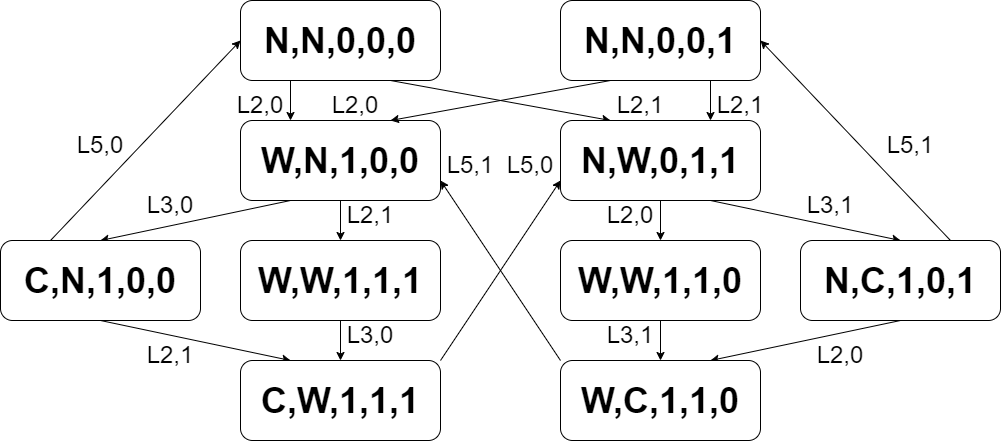
\includegraphics[width=0.8\textwidth]{image/hw1-3-1.drawio.png}
    \caption{State Transition Graph for Part 1}
    \label{fig:hw1-3-1}
\end{figure}

\subsection{Part 2}

As you can see in the image, there is not a state where $C_0$ and $C_1$ happen at the same time.

\section{Problem 4}

\subsection{Part 1}

Example of a iteration:

\begin{enumerate}
    \item Before start of the iteration:
        $y_1 = 0$ and $y_2 = x$.
        $P_1$ is about to execute $y_1 = y_2 + 1$.
        $P_2$ is about to execute $y_2 = 0$.
    \item $P_1$ executes $y_1 = y_2 + 1$.
        Now $y_1 = x + 1, y_2 = x$.
    \item $P_2$ executes $y_2 = 0$ (finishes the critical section).
        Now $y_1 = x + 1, y_2 = 0$.
    \item $P_2$ executes $y_2 = y_1 + 1$.
        Now $y_1 = x + 1, y_2 = x + 2$.
    \item $P_1$ tests $y_2 = 0 \vee y_1 < y_2$.
        It is true, so $P_1$ enters the critical section.
    \item $P_1$ finishes the critical section, and set $y_1 = 0$.
        Now $y_1 = 0, y_2 = x + 2$.
    \item $P_2$ tests $y_1 = 0 \vee y_2 < y_1$.
        It is true, so $P_2$ enters the critical section.
    \item Now, $P_1$ is about to execute $y_1 = y_2 + 1$,
        and $P_2$ is about to execute $y_2 = 0$, the start of another iteration.
\end{enumerate}

As long as we can reach the start of some iteration, we can get into an infinite loop.
During each iteration, the value of $y_2$ will grow by $2$, which indicates an infinite transition system,
since the state of the system is unbounded.

So, we just need to prove that we can arrive at the start of some iteration.

Consider the following steps:

\begin{enumerate}
    \item At first, $y_1 = y_2 = 0$.
    \item $P_2$ executes $y_2 = y_1 + 1$.
        Now $y_1 = 0, y_2 = 1$.
    \item $P_2$ tests $y_1 = 0 \vee y_2 < y_1$.
        It is true, so $P_2$ enters the critical section.
    \item Now, it is the start of an iteration where $x = 1$.
\end{enumerate}

In conlusion, the value of $y_2$ can grow arbitrarily large, resulting in an infinite transition system.

\subsection{Part 2}

Proof by contradiction. If both $P_1$ and $P_2$ enters the critical section, then we have:

$$
(y_2 = 0 \vee y_1 < y_2) \wedge (y_1 = 0 \vee y_2 < y_1)
$$

Since at most one in $y_1 < y_2$ and $y_2 < y_1$ can be true, we have at least $y_1 = 0$ or $y_2 = 0$.
Due to the symmetry of the two programs, without loss of generality, we assume $y_2 = 0$.

First of all, it's trivial to see $y_1 \ge 0$ and $y_2 \ge 0$, which can be proved by induction
(each write to $y_1$ or $y_2$ is non-negative, whatever the sequence of the writes is).

In addition, the last write to $y_2$ before $P_2$ enters the critical section is $y_2 = y_1 + 1$,
so we have $y_2 \ge 0 + 1 = 1$, which contradicts the assumption $y_2 = 0$.

As a result, we have proved that $P_1$ and $P_2$ cannot enter the critical section at the same time.
